\section{Граф взаимодействия переменных. Partition Crossover}
\subsection{Граф взаимодействия переменных.}
Продолжаем рассматривать оптимизацию серого ящика, помним о том, что у нас есть некоторое представление о том как происходит получение результата в процессе работы над аргументами. Теперь построим граф взаимодействия переменных.
\begin{itemize}
    \item Вершины соответствуют переменным
    \item $x_1$ и $x_2$ соединены ребром, если они взаимодействуют нелинейным образом, то есть, существует какая то подфункция $f_i $зависящая и от $x_1$ и от $x_2$
\end{itemize}
Как вы думаете, что будет, если граф взаимодействия переменных будет ацикличным? т.е. не будет попарно связных ребер. О чем это может говорить?\\
Если у нас есть некоторые "висящие"(?) переменные и их весьма много, то такой граф выродится в ациклический. И это говорит о том, что либо эти переменные взаимодействуют только с одним критерием оставшихся переменных отбора функции. Есть такие критерии, по которым можно определить, что переменные взаимодействуют с только одного характера переменными для вычисления подфункции. Либо эти переменные вообще константные\\
\begin{figure}[h]
\centering
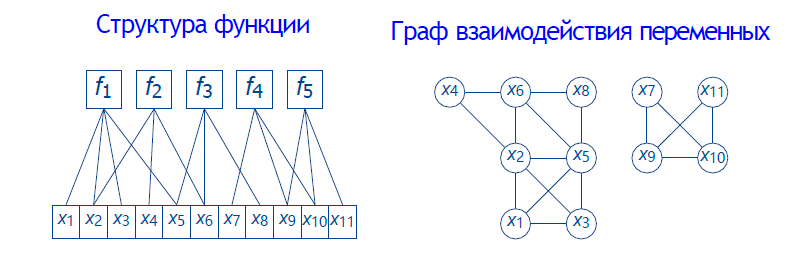
\includegraphics[width=0.8\linewidth]{images/graf.PNG}
\end{figure}
Для k ограниченных функций с m подфункциями, число ребер в VIG составляет $O(k^2m)$. Имеется ввиду количество нелинейных зависимостей между переменных.
\subsection{Partition Crossover}

При рассмотрении функции серого ящика и при представлении функций и переменных в графе взаимодействия мы можем рассмотреть Partition Crossover.\\
\begin{itemize}
    \item Пусть у нас есть две битовые строки, являющиеся локальными оптимумами при некотором определении локальности. т.е. известно что для данного серого ящика накладываются ограничения, которые делают выбранное пространство локальным и есть некие заданные некоторый локальный оптимум.
    \item Найдем переменные с совпадающими значениями, удалим их из VIG(графа взаимодействия)
    \item Найдем лучшую из двух битовых подпоследовательностей для каждой компоненты связности независимо.
    \item Результат тоже будет (хорошим!) локальным оптимумом для каждой особи
\end{itemize}

\textbf{Пример}\\
\begin{figure}[h]
\centering
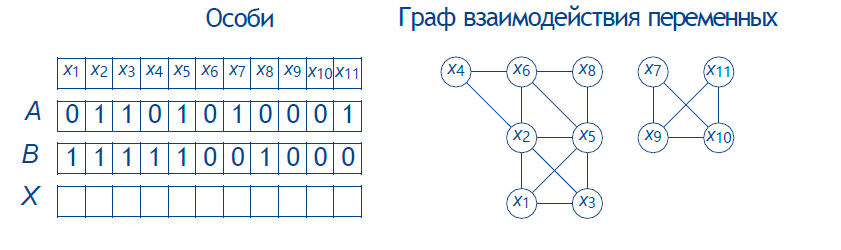
\includegraphics[width=0.8\linewidth]{images/pc1.PNG}
\end{figure}
Слева - особь, А,В - заданные локальные оптимумы. Справа - задан граф взаимодействия. Далее нам надо найти элементы с повторяющимеся значениями и удалить из графа взаимодействия переменных подфункций. \\
Находим:\\
Смотрим на переменные $x_2,x_3,x_5,x_6$ они связанымежду собой нелинейным взаимодействием. $x_9,x_{10}$ - тоже самое.\\
\begin{figure}[h]
\centering
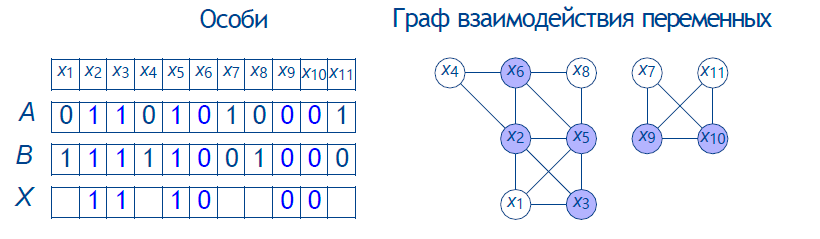
\includegraphics[width=0.8\linewidth]{images/pc3.PNG}
\end{figure}
Далее найдем лучшую из двух битовых подпоследовательностей для каждой компоненты $x_1, x_4,x_7,x_8 x_{11}$. Получилась битовая строка $X$, которая представляет собой локальный оптимум для нашего решения.\\
Что будет если провести ребро между $x_{11}$ и $x_7$? Как бы изменилась строка? \\
Тогда мы бы также удалили эти вершины.\\
\begin{figure}[h]
\centering
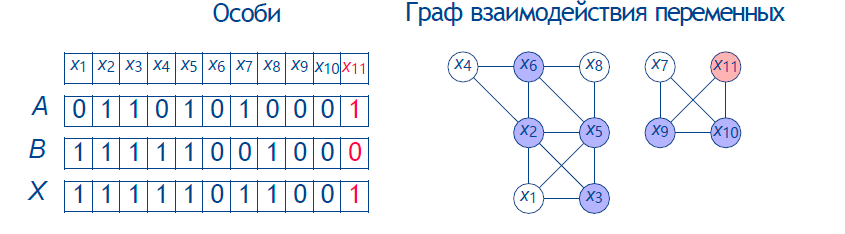
\includegraphics[width=0.8\linewidth]{images/pc11.PNG}
\end{figure}

\textbf{PartitionCrossover: эксперименты}\\
Простой генетический алгоритм
\begin{itemize}
    \item Размер популяции 50, вероятность мутации $\frac{1}{n}$ 100 поколений, усреднение по 50 экспериментам
    \item Используются различные операторы скрещивания: двухточечный, однородный, partition crossover
\end{itemize}

Задачи оптимизации
\begin{itemize}
    \item NK-ландшафты: смежные (простые задачи), случайные (сложные задачи)
    \item $K\in{1,2,3}, N=500 $, N - итерации, К-ограничение на кол-во переменных
\end{itemize}

Доля новых особей, являющихся локальными оптимумами\\
\begin{figure}[h]
\centering
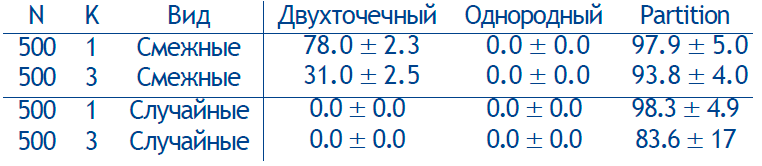
\includegraphics[width=0.8\linewidth]{images/tbl.PNG}
\end{figure}
Число компонент связности в Partition Crossover\\
\begin{figure}[h]
\centering
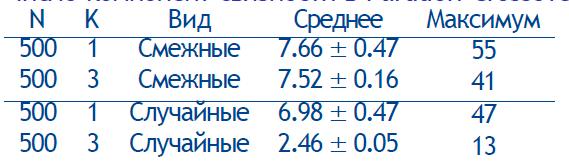
\includegraphics[width=0.8\linewidth]{images/tbl2.PNG}
\end{figure}
Есть некоторая кореляция между значениями компонент связности и значением оператора Partition. Чем выше среднее, тем выше количество нелинейно зависимых переменных. Для минимального значения K, получаем максимальное значения NK-ландшафтов. 
Смежные NK-ландшафты, доля оптимальных решений\\
\begin{figure}[h]
\centering
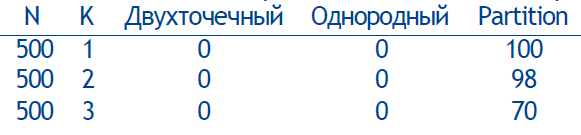
\includegraphics[width=0.8\linewidth]{images/tbl3.PNG}
\end{figure}
Случайные NK-ландшафты, средняя нормализованная приспособленность. При нормализации получаем свежие значения путем адаптации значений. В данном случае можно выкинть однородный оператор т.к. он ни на что не повлияет\\
\begin{figure}[h]
\centering
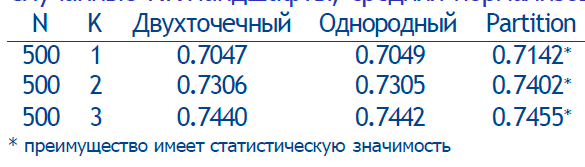
\includegraphics[width=0.8\linewidth]{images/tbl4.PNG}
\end{figure}
